\documentclass[14pt,ignorenonframetext]{beamer}
\setbeamertemplate{caption}[numbered]
\setbeamertemplate{caption label separator}{:}
\setbeamercolor{caption name}{fg=normal text.fg}
\usepackage{amssymb,amsmath}
\usepackage{ifxetex,ifluatex}
\usepackage{fixltx2e} % provides \textsubscript
\usepackage{lmodern}
\ifxetex
  \usepackage{fontspec,xltxtra,xunicode}
  \defaultfontfeatures{Mapping=tex-text,Scale=MatchLowercase}
  \newcommand{\euro}{€}
\else
  \ifluatex
    \usepackage{fontspec}
    \defaultfontfeatures{Mapping=tex-text,Scale=MatchLowercase}
    \newcommand{\euro}{€}
  \else
    \usepackage[T1]{fontenc}
    \usepackage[utf8]{inputenc}
      \fi
\fi
% use upquote if available, for straight quotes in verbatim environments
\IfFileExists{upquote.sty}{\usepackage{upquote}}{}
% use microtype if available
\IfFileExists{microtype.sty}{\usepackage{microtype}}{}
\usepackage{url}

% Comment these out if you don't want a slide with just the
% part/section/subsection/subsubsection title:
\AtBeginPart{
  \let\insertpartnumber\relax
  \let\partname\relax
  \frame{\partpage}
}
\AtBeginSection{
  \let\insertsectionnumber\relax
  \let\sectionname\relax
  \frame{\sectionpage}
}
\AtBeginSubsection{
  \let\insertsubsectionnumber\relax
  \let\subsectionname\relax
  \frame{\subsectionpage}
}

\setlength{\parindent}{0pt}
\setlength{\parskip}{6pt plus 2pt minus 1pt}
\setlength{\emergencystretch}{3em}  % prevent overfull lines
\setcounter{secnumdepth}{0}
% Thanks Richard Darst on how to get a nice Beamer theme.
% See http://rkd.zgib.net/wiki/DebianBeamerThemes

\usepackage{ctable}
\usepackage{multicol}
\usepackage{tikz}

%\usebackgroundtemplate{
\includegraphics[width=\paperwidth]{images/swirl-lightest.pdf}}
%\logo{
\includegraphics[viewport=274 335 360 440,width=1cm]{images/openlogo-nd.pdf}}

\definecolor{debianred}{rgb}{.780,.000,.211} % 199,0,54
\definecolor{debianblue}{rgb}{0,.208,.780} % 0,53,199
\definecolor{debianlightbackgroundblue}{rgb}{.941,.941,.957} % 240,240,244
\definecolor{debianbackgroundblue}{rgb}{.776,.784,.878} % 198,200,224

\usetheme{Boadilla}
\setbeamertemplate{navigation symbols}{}

\usecolortheme[named=debianbackgroundblue]{structure}
\setbeamercolor{normal text}{fg=black}
\setbeamercolor{titlelike}{fg=debianblue}
\setbeamercolor{sidebar}{fg=debianred,bg=debianbackgroundblue}

\setbeamercolor{palette sidebar primary}{fg=debianred}
\setbeamercolor{palette sidebar secondary}{fg=debianred}
\setbeamercolor{palette sidebar tertiary}{fg=debianred}
\setbeamercolor{palette sidebar quaternary}{fg=debianred}

\setbeamercolor{section in toc}{fg=debianred}
\setbeamercolor{subsection in toc}{parent=debianred}

\setbeamercolor{item}{fg=debianred}

\setbeamercolor{block title}{fg=debianblue}

\title[Reproducible builds HOWTO]{How to make your software build reproducibly}
\subtitle{Provide a verifiable path from source to binary}
\author[Lunar]{%
   \texorpdfstring{
            Lunar\\
            \href{mailto:lunar@debian.org}{lunar@debian.org}
   }{Lunar}}
\institute[Debian]{}
\date[CCCamp15]{%
 Chaos Communication Camp\\
 \small
 2015-08-13}

\begin{document}

\begin{frame}

\titlepage

\end{frame}

\section{Introduction}

\begin{frame}
\frametitle{The problem}

\center

\begin{tikzpicture}
\draw (-2,0) node[font=\LARGE] (source) { source };
\draw (2,0) node[font=\LARGE] (binary) { binary };
\draw[->,very thick] (source) -- (binary) node[midway] (midbuild) {};
\draw (midbuild) node [above,color=debianred,font=\small] (build) {build};
\visible<2>{
\draw (0,2) node[font=\LARGE,color=debianblue] (fs) { free software };
% font= specification is required to work-around a bug in md->latex conversion
\draw[->,font=\normalsize] (fs) -- (source) node[midway,left=0.2cm,color=debianred,font=\footnotesize,align=center]{freedom\\to study};
\draw[->,font=\normalsize] (fs) -> (binary) node[midway,right=0.2cm,color=debianred,font=\footnotesize,align=center]{freedom\\to run};
}
\visible<3->{
\draw (-4,-1) node[font=\small,color=debianblue] (verified) { can be verified };
\draw (4,-1) node[font=\small,color=debianblue] (used) { can be used };
\path (verified) edge[->,bend left=30] (source);
\path (used) edge[->,bend right=30] (binary);
}
\visible<4->{
\draw (0,-2) node[font=\LARGE,color=debianred,align=center] (prove) { could I get a proof? };
\path (prove) edge[->] (midbuild);
}
\end{tikzpicture}

\end{frame}

\begin{frame}
\frametitle{Why does it matter?}

Mike Perry and Seth Schoen at 31C3: Reproducible builds

XXX: verify, provide URL

\end{frame}

\begin{frame}[fragile]
\frametitle{Just one example}

At a CIA conference in 2012:

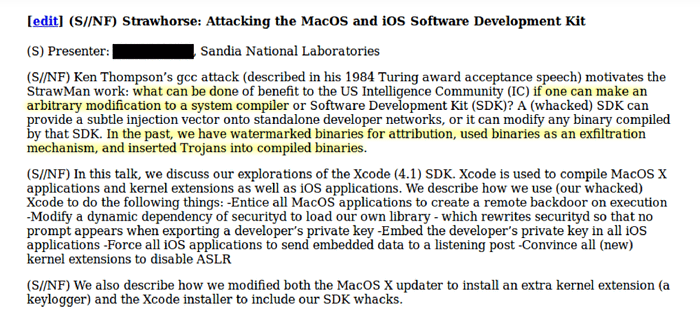
\includegraphics[width=\textwidth]{images/strawhorse}

Source~: The Intercept, 2015-03-10
\url{https://firstlook.org/theintercept/2015/03/10/ispy-cia-campaign-steal-apples-secrets/}

\end{frame}

\begin{frame}
\frametitle{The solution}

\begin{center}
\Large
enable anyone to reproduce\\
identical binary packages\\
from a given source
\end{center}

\end{frame}

\begin{frame}
\frametitle{The solution}

We call this:

\begin{center}
\Huge
“reproducible builds”
\end{center}

\end{frame}

\begin{frame}
\frametitle{It's trendy!}

\begin{itemize}
\item Bitcoin (\textbf{done})
\item Tor (\textbf{done})
\item Debian (\emph{in progress})
\item FreeBSD (\emph{in progress})
\item Coreboot (\textbf{done})
\item OpenWrt (\emph{in progress})
\item \ldots{}
\end{itemize}

\end{frame}

\begin{frame}
\frametitle{Multiple aspects}

\begin{itemize}
\item Deterministic build system \\
  \textit{\small for those who write source code}
\item Reproducible build environment \\
  \textit{\small for those who create binaries for others}
\item Distributing the build environment \\
  \textit{\small for those who distribute binaries to the world}
\end{itemize}

\end{frame}

\section{Deterministic build system}

\begin{frame}
\frametitle{Deterministic build system}

In a nutshell:

\begin{itemize}
\item Stable inputs
\item Stable outputs
\item Capture as little as possible from the environment
\end{itemize}

\end{frame}

\begin{frame}
\frametitle{Volatile inputs can disappear}

\begin{itemize}
\item Don't rely on the network
\item If you do, have a backup
\item The binary distributor should provide a fallback
\end{itemize}

XXX: add an example from FreeBSD port tree

\end{frame}

\begin{frame}[fragile]
 \frametitle{Stable order for inputs}

 \begin{overprint}
  \onslide<1>
  \begin{itemize}
   \item Always process multiple inputs in the same order
   \item Directory listings are not stable!
  \end{itemize}

  \onslide<2>
  \begin{itemize}
   \item List inputs explicitely
  \end{itemize}

  \onslide<3->
  \begin{itemize}
   \item Use sorting
   \item<4> \alert{But watch out for difference between locales.}
  \end{itemize}
 \end{overprint}

 \begin{overprint}
  \onslide<1>
  \begin{block}{Bad example}
\begin{semiverbatim}
tar -cf archive.tar src
\end{semiverbatim}
  \end{block}

  \onslide<2>
  \begin{block}{Good example}
\begin{semiverbatim}
tar -cf archive.tar \\
  src/util.c src/helper.c src/main.c
\end{semiverbatim}
  \end{block}

  \onslide<3->
  \begin{block}{Good example}
\begin{semiverbatim}
find src -print0 | \only<4>{\alert{LC\_ALL=C} }sort -z  |
    tar --null -T - --no-recursion -cf archive.tar
\end{semiverbatim}
  \end{block}
 \end{overprint}
\end{frame}

\begin{frame}
 \frametitle{Controlled value initialization}

 \begin{itemize}
  \item Don't record memory by accident
  \item<2>Always initialize to a known value
 \end{itemize}

 \begin{example}
\begin{semiverbatim}
    XXX: insert Coreboot example
\end{semiverbatim}
 \end{example}
\end{frame}

\begin{frame}
 \frametitle{Use deterministic version information}

 \begin{itemize}
  \item Don't make a version number on each build
  \item<2> Instead extract information from the source:
    \begin{itemize}
      \item Version control system revision
      \item Hash of the source code
      \item Changelog entry
    \end{itemize}
 \end{itemize}

 XXX: example
\end{frame}

\begin{frame}
 \frametitle{Don't record the current date and time}

 \begin{itemize}
  \item Avoid timestamps
  \item<2-> If you need one:
    \begin{itemize}
      \item Use date of last commit in VCS
      \item Extract from changelog
      \item<3-> \alert{Don't forget the timezone}
    \end{itemize}
  \item<4> Implement \texttt{SOURCE\_DATE\_EPOCH} \\
    \url{https://wiki.debian.org/ReproducibleBuilds/TimestampsProposal}
 \end{itemize}
\end{frame}

\begin{frame}[fragile]
 \frametitle{Don't record current time (really)}

 \begin{itemize}
  \item Archives keep modification times in metadata
  \item Storing a file can record build time
  \item<2-> Solutions:
   \begin{itemize}
    \item Store an arbitrary value
    \item<3-> Pre-process file modification time
    \item<4> Post-process archive
   \end{itemize}
 \end{itemize}

 \begin{example}
\begin{semiverbatim}
\visible<3>{\alert{touch --date="2015-08-13 00:00Z" build/*}}
tar\only<2>{\alert{ --mtime='2015-08-13 00:00Z'}} -cf product.tar build
\visible<4>{\alert{strip-nondeterminism product.tar}}
\end{semiverbatim}
 \end{example}
\end{frame}

\begin{frame}[fragile]
 \frametitle{Stable order for outputs}

 \begin{itemize}
  \item Always output lists in the same order
  \item Typical issue: key order with hash tables
  \item<2> Sort!
 \end{itemize}

 \begin{example}
\begin{semiverbatim}
for module in \only<2>{\alert{sorted(}}dependencies.keys()\only<2>{\alert{)}}:
    version = dependencies[module]
    print('\%s (>= \%s)' \% (module, version))
\end{semiverbatim}
 \end{example}
\end{frame}

\begin{frame}[fragile]
 \frametitle{Avoid (true) randomness}

 \begin{itemize}
  \item Randomness is not deterministic
  \item<2-> Seed for your PRNG from known value
   \begin{itemize}
     \item Use a fixed value
     \item<3> Extract from source code
   \end{itemize}
 \end{itemize}

 \begin{example}
\begin{semiverbatim}\small
CFLAGS="-O2\only<2->{ \alert{-frandom-seed=}}\only<2>{\alert{0}}\only<3>{\alert{\$(git rev-parse HEAD)}}"
gcc -c utils.c
\end{semiverbatim}
 \end{example}

 XXX: find an example of how gcc uses -frandom-seed
\end{frame}

\begin{frame}
 \frametitle{Define environment variable affecting outputs}

 \begin{itemize}
  \item Some environment variables will affect software outputs. E.g:
   \begin{itemize}
    \item \texttt{LC\_CTIME} for time strings
    \item \texttt{LC\_CTYPE} for text encoding
    \item \texttt{TZ} for times
   \end{itemize}
  \item<2-> Set them to a controlled value
  \item<3> \textit{Please don't force the language}
 \end{itemize}
\end{frame}

\begin{frame}
 \frametitle{Stop recording build system information}

 \begin{itemize}
  \item Don't record information about the build system, like:
   \begin{itemize}
    \item date and time of the build
    \item hostname
    \item path
    \item network configuration
    \item CPU
    \item environment variables
    \item …
   \end{itemize}
  \item<2> If you really want to record them, do it outside the binaries
 \end{itemize}
\end{frame}

\section{Reproducible build environment}

\begin{frame}
 \frametitle{What's a build environment?}

 \begin{itemize}
  \item Toolchain
  \item XXX: research Tor Browser / Bitcoin
  \item \textit{Build patd}
  \item \textit{Build date and time}
 \end{itemize}
\end{frame}

\begin{frame}
 \frametitle{Build from source}

 \begin{itemize}
  \item Coreboot
  \item OpenWrt ?
 \end{itemize}
\end{frame}

\begin{frame}
 \frametitle{Good old Makefile}

 \begin{itemize}
  \item \texttt{make env} XXX: research Coreboot and OpenWrt
  \item Download known toolchain archive
  \item Compare reference checksums
  \item Build and setup
 \end{itemize}
\end{frame}

\begin{frame}
 \frametitle{Google approach}

 XXX: go ask people

 \begin{itemize}
  \item Check-in toolchain source code in VCS
  \item Find toolchain change causing regressions
  \item See Bazel \\
   \url{https://bazel.io/} XXX: check URL
 \end{itemize}
\end{frame}

\begin{frame}
 \frametitle{Reference distribution}

 \begin{itemize}
  \item Use a stable distribution (e.g. Debian, CentOS) XXX: demander à misc
  \item Record package version
 \end{itemize}
\end{frame}

\begin{frame}
 \frametitle{Proprietary operating systems}

 \begin{itemize}
  \item Cross-compiling to the rescue!
  \item For Windows:
   \begin{itemize}
     \item MingW64 XXX: research
     \item NSIS Installer
   \end{itemize}
  \item For Mac OS X:
   \begin{itemize}
     \item hacked xcode XXX: research
     \item DMG XXX
   \end{itemize}
 \end{itemize}
\end{frame}

\section{Distributing the build environment}

\begin{frame}
 \frametitle{OpenWrt}

 XXX: research
\end{frame}

\begin{frame}
 \frametitle{Gitian}

\end{frame}

\begin{frame}
 \frametitle{Docker}

\end{frame}

\begin{frame}
 \frametitle{Debian .buildinfo}

 XXX: explain
\end{frame}

\section{Tips}

\begin{frame}
 \frametitle{Debbuging}

 XXX diffoscope
\end{frame}

\begin{frame}
 \frametitle{diffoscope example}
\end{frame}

\begin{frame}
 \frametitle{reproducible.debian.net}

\end{frame}

\begin{frame}
 \frametitle{strip-nondeterminism}

\end{frame}

\begin{frame}
 \frametitle{Resources}

 \begin{itemize}
  \item Debian “Reproducible Builds” wiki \\
   \url{https://wiki.debian.org/ReproducibelBuilds}
  \item Diverse Double Compilation XXX
 \end{itemize}
\end{frame}

\section{Question?}

\begin{frame}
 \frametitle{Thanks!}

 \begin{itemize}
  \item Debian “Reproducible Builds” team \\
    {\small (you are just \textbf{so} awesome!)}
  \item Mike Perry, Georg Koppen
  \item David A. Wheeler
  \item Linux Foundation
 \end{itemize}

 \begin{center}
  \begin{tabular}{rl}
   OpenPGP & \texttt{0603 CCFD 9186 5C17 E88D} \\
           & \texttt{4C79 8382 C95C 2902 3DF9}
  \end{tabular}

 \begin{center}\small
  Clothes: Elhonna Sombrefeuille — Hair: igor
 \end{center}

 \end{center}
\end{frame}

\end{document}
